\documentclass{standalone}

\usepackage{tikz}

\begin{document}
  %noformat{
  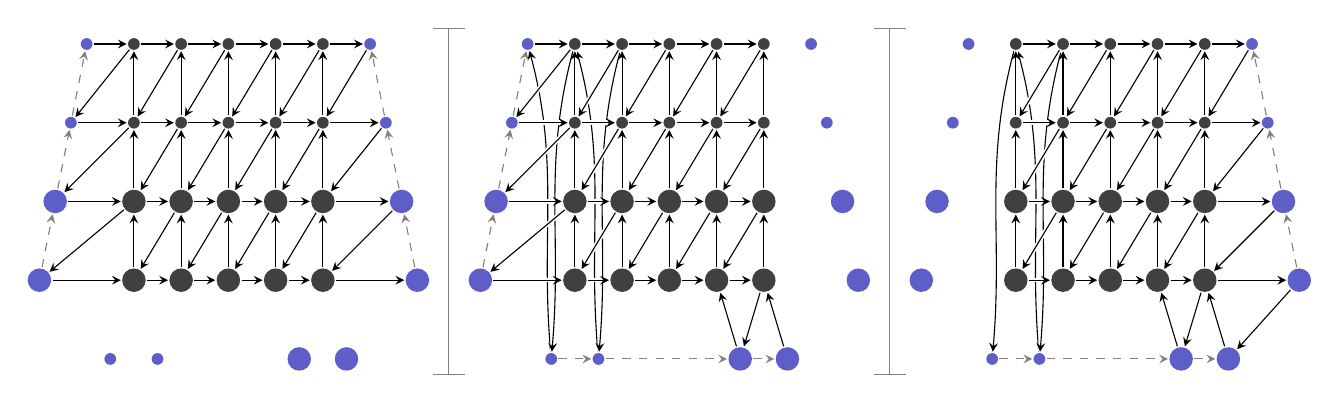
\begin{tikzpicture}
    \tikzstyle{v1} = [circle, outer sep=0.5pt, fill, inner sep=1.5pt]
    \tikzstyle{v2} = [circle, outer sep=0.5pt, fill, inner sep=3.0pt]
    \tikzstyle{unf} = [color=darkgray]
    \tikzstyle{frz} = [color=blue!60!darkgray!70]
    \tikzstyle{e} = [->, >={stealth}, preaction={draw=white, -, ultra thick}]
    \tikzstyle{r} = [color=red!70!darkgray!70]
    \tikzstyle{h} = [dashed, color=gray, ->, >={stealth}]

    % Q_0
    \begin{scope}[shift={(0,0)}]
      \node[v2, frz] (v16) at (-0.6,0) {};
      \node[v2, frz] (v26) at (-0.4,1) {};
      \node[v1, frz] (v36) at (-0.2,2) {};
      \node[v1, frz] (v46) at ( 0.0,3) {};

      \node[v2, unf] (v15) at (0.6,0) {};
      \node[v2, unf] (v25) at (0.6,1) {};
      \node[v1, unf] (v35) at (0.6,2) {};
      \node[v1, unf] (v45) at (0.6,3) {};

      \node[v2, unf] (v14) at (1.2,0) {};
      \node[v2, unf] (v24) at (1.2,1) {};
      \node[v1, unf] (v34) at (1.2,2) {};
      \node[v1, unf] (v44) at (1.2,3) {};

      \node[v2, unf] (v13) at (1.8,0) {};
      \node[v2, unf] (v23) at (1.8,1) {};
      \node[v1, unf] (v33) at (1.8,2) {};
      \node[v1, unf] (v43) at (1.8,3) {};

      \node[v2, unf] (v12) at (2.4,0) {};
      \node[v2, unf] (v22) at (2.4,1) {};
      \node[v1, unf] (v32) at (2.4,2) {};
      \node[v1, unf] (v42) at (2.4,3) {};

      \node[v2, unf] (v11) at (3.0,0) {};
      \node[v2, unf] (v21) at (3.0,1) {};
      \node[v1, unf] (v31) at (3.0,2) {};
      \node[v1, unf] (v41) at (3.0,3) {};

      \node[v2, frz] (v10) at (4.2,0) {};
      \node[v2, frz] (v20) at (4.0,1) {};
      \node[v1, frz] (v30) at (3.8,2) {};
      \node[v1, frz] (v40) at (3.6,3) {};

      \node[v2, frz] (A1) at (3.3,-1) {};
      \node[v2, frz] (A2) at (2.7,-1) {};
      \node[v1, frz] (A3) at (0.9,-1) {};
      \node[v1, frz] (A4) at (0.3,-1) {};

      \foreach \p in {0, 6} {
        \draw[h] (v1\p) -- (v2\p);
        \draw[h] (v2\p) -- (v3\p);
        \draw[h] (v3\p) -- (v4\p);
      }
      \foreach \p in {1, 2, 3, 4, 5} {
        \draw[e] (v1\p) -- (v2\p);
        \draw[e] (v2\p) -- (v3\p);
        \draw[e] (v3\p) -- (v4\p);
      }
      \foreach \p/\q in {0/1, 1/2, 2/3, 3/4, 4/5, 5/6} {
        \draw[e] (v1\q) -- (v1\p);
        \draw[e] (v2\q) -- (v2\p);
        \draw[e] (v3\q) -- (v3\p);
        \draw[e] (v4\q) -- (v4\p);
        \draw[e] (v2\p) -- (v1\q);
        \draw[e] (v3\p) -- (v2\q);
        \draw[e] (v4\p) -- (v3\q);
      }
    \end{scope}

    \draw[gray, thin] ( 4.6,-1.2) -- ( 4.6, 3.2);
    \draw[gray, thin] ( 4.4, 3.2) -- ( 4.8, 3.2);
    \draw[gray, thin] ( 4.4,-1.2) -- ( 4.8,-1.2);

    % Q_0'
    \begin{scope}[shift={(5.6,0)}]
      \node[v2, frz] (v16) at (-0.6,0) {};
      \node[v2, frz] (v26) at (-0.4,1) {};
      \node[v1, frz] (v36) at (-0.2,2) {};
      \node[v1, frz] (v46) at ( 0.0,3) {};

      \node[v2, unf] (v15) at (0.6,0) {};
      \node[v2, unf] (v25) at (0.6,1) {};
      \node[v1, unf] (v35) at (0.6,2) {};
      \node[v1, unf] (v45) at (0.6,3) {};

      \node[v2, unf] (v14) at (1.2,0) {};
      \node[v2, unf] (v24) at (1.2,1) {};
      \node[v1, unf] (v34) at (1.2,2) {};
      \node[v1, unf] (v44) at (1.2,3) {};

      \node[v2, unf] (v13) at (1.8,0) {};
      \node[v2, unf] (v23) at (1.8,1) {};
      \node[v1, unf] (v33) at (1.8,2) {};
      \node[v1, unf] (v43) at (1.8,3) {};

      \node[v2, unf] (v12) at (2.4,0) {};
      \node[v2, unf] (v22) at (2.4,1) {};
      \node[v1, unf] (v32) at (2.4,2) {};
      \node[v1, unf] (v42) at (2.4,3) {};

      \node[v2, unf] (v11) at (3.0,0) {};
      \node[v2, unf] (v21) at (3.0,1) {};
      \node[v1, unf] (v31) at (3.0,2) {};
      \node[v1, unf] (v41) at (3.0,3) {};

      \node[v2, frz] (v10) at (4.2,0) {};
      \node[v2, frz] (v20) at (4.0,1) {};
      \node[v1, frz] (v30) at (3.8,2) {};
      \node[v1, frz] (v40) at (3.6,3) {};

      \node[v2, frz] (A1) at (3.3,-1) {};
      \node[v2, frz] (A2) at (2.7,-1) {};
      \node[v1, frz] (A3) at (0.9,-1) {};
      \node[v1, frz] (A4) at (0.3,-1) {};

      \draw[h] (A4) -- (A3);
      \draw[h] (A3) -- (A2);
      \draw[h] (A2) -- (A1);

      \draw[e] (A4)  to[out= 95,in=285] (v46);
      \draw[e] (v45) to[out=255,in= 85] (A4);
      \draw[e] (A3)  to[out= 95,in=285] (v45);
      \draw[e] (v44) to[out=255,in= 85] (A3);
      \draw[e] (A2) -- (v12);
      \draw[e] (v11) -- (A2);
      \draw[e] (A1) -- (v11);

      \foreach \p in {6} {
        \draw[h] (v1\p) -- (v2\p);
        \draw[h] (v2\p) -- (v3\p);
        \draw[h] (v3\p) -- (v4\p);
      }
      \foreach \p in {1, 2, 3, 4, 5} {
        \draw[e] (v1\p) -- (v2\p);
        \draw[e] (v2\p) -- (v3\p);
        \draw[e] (v3\p) -- (v4\p);
      }
      \foreach \p/\q in {1/2, 2/3, 3/4, 4/5, 5/6} {
        \draw[e] (v1\q) -- (v1\p);
        \draw[e] (v2\q) -- (v2\p);
        \draw[e] (v3\q) -- (v3\p);
        \draw[e] (v4\q) -- (v4\p);
        \draw[e] (v2\p) -- (v1\q);
        \draw[e] (v3\p) -- (v2\q);
        \draw[e] (v4\p) -- (v3\q);
      }

    \end{scope}

    \draw[gray, thin] (10.2,-1.2) -- (10.2, 3.2);
    \draw[gray, thin] (10.0, 3.2) -- (10.4, 3.2);
    \draw[gray, thin] (10.0,-1.2) -- (10.4,-1.2);

    % Q_0''
    \begin{scope}[shift={(11.2,0)}]
      \node[v2, frz] (v16) at (-0.6,0) {};
      \node[v2, frz] (v26) at (-0.4,1) {};
      \node[v1, frz] (v36) at (-0.2,2) {};
      \node[v1, frz] (v46) at ( 0.0,3) {};

      \node[v2, unf] (v15) at (0.6,0) {};
      \node[v2, unf] (v25) at (0.6,1) {};
      \node[v1, unf] (v35) at (0.6,2) {};
      \node[v1, unf] (v45) at (0.6,3) {};

      \node[v2, unf] (v14) at (1.2,0) {};
      \node[v2, unf] (v24) at (1.2,1) {};
      \node[v1, unf] (v34) at (1.2,2) {};
      \node[v1, unf] (v44) at (1.2,3) {};

      \node[v2, unf] (v13) at (1.8,0) {};
      \node[v2, unf] (v23) at (1.8,1) {};
      \node[v1, unf] (v33) at (1.8,2) {};
      \node[v1, unf] (v43) at (1.8,3) {};

      \node[v2, unf] (v12) at (2.4,0) {};
      \node[v2, unf] (v22) at (2.4,1) {};
      \node[v1, unf] (v32) at (2.4,2) {};
      \node[v1, unf] (v42) at (2.4,3) {};

      \node[v2, unf] (v11) at (3.0,0) {};
      \node[v2, unf] (v21) at (3.0,1) {};
      \node[v1, unf] (v31) at (3.0,2) {};
      \node[v1, unf] (v41) at (3.0,3) {};

      \node[v2, frz] (v10) at (4.2,0) {};
      \node[v2, frz] (v20) at (4.0,1) {};
      \node[v1, frz] (v30) at (3.8,2) {};
      \node[v1, frz] (v40) at (3.6,3) {};

      \node[v2, frz] (A1) at (3.3,-1) {};
      \node[v2, frz] (A2) at (2.7,-1) {};
      \node[v1, frz] (A3) at (0.9,-1) {};
      \node[v1, frz] (A4) at (0.3,-1) {};

      \draw[h] (v10) -- (v20);
      \draw[h] (v20) -- (v30);
      \draw[h] (v30) -- (v40);
      \draw[h] (A4) -- (A3);
      \draw[h] (A3) -- (A2);
      \draw[h] (A2) -- (A1);

      \draw[e] (v45) to[out=255,in= 85] (A4);
      \draw[e] (A3)  to[out= 95,in=285] (v45);
      \draw[e] (v44) to[out=255,in= 85] (A3);
      \draw[e] (A2) -- (v12);
      \draw[e] (v11) -- (A2);
      \draw[e] (A1) -- (v11);
      \draw[e] (v10) -- (A1);

      \foreach \p in {1, 2, 3, 4, 5} {
        \draw[e] (v1\p) -- (v2\p);
        \draw[e] (v2\p) -- (v3\p);
        \draw[e] (v3\p) -- (v4\p);
      }
      \foreach \p/\q in {0/1, 1/2, 2/3, 3/4, 4/5} {
        \draw[e] (v1\q) -- (v1\p);
        \draw[e] (v2\q) -- (v2\p);
        \draw[e] (v3\q) -- (v3\p);
        \draw[e] (v4\q) -- (v4\p);
        \draw[e] (v2\p) -- (v1\q);
        \draw[e] (v3\p) -- (v2\q);
        \draw[e] (v4\p) -- (v3\q);
      }
    \end{scope}

  \end{tikzpicture}
  %}noformat
\end{document}
